\chapter{Introduction}

During the last decades, observations of low-energy extraterrestrial neutrinos have pushed forward our understanding of astrophysical environments and elucidated properties of neutrinos.
Measurements of $\si\MeV$ neutrinos from the Sun, the closest detected extraterrestrial neutrino source, have led to an improved understanding of the Sun's inner workings~\cite{Raffelt:1999tx,Bahcall:2004pz} and have been pivotal in resolving the neutrino flavor-changing puzzle~\cite{McDonald:2016ixn}.
Similarly, the observation of neutrinos from supernova 1987a~\cite{Hirata:1987hu,Bratton:1988ww}, in the Large Magellanic Cloud, has provided irreplaceable information for supernovae physics~\cite{Bethe:1990mw}, as well as important constraints of neutrino properties~\cite{Arnett:1987iz,Goldman:1987fg,Manohar:1987ec,Lattimer:1988mf} and fundamental physics~\cite{Raffelt:1987yt,Turner:1987by}.

We now look to the new frontier of high-energy extraterrestrial neutrino physics that has been opened by the IceCube, with the hope that we may repeat success others have had at lower energies.
The origin of cosmic rays has been a long standing problem in astrophysics, which we have been unable to resolve with measurements of cosmic rays alone.
High-energy neutrinos are expected to be produced in hadronic processes that are likely to occur near sites of cosmic ray acceleration.
This process of neutrino production makes regions of charged-particle acceleration prime candidates as high-energy neutrino sources, and in turn may allow us to use neutrinos to probe the issue of cosmic ray origin.

A variety of astrophysical objects are capable of accelerating cosmic rays to extremely high energies.
When these cosmic-rays interact with material or radiation near the acceleration region, particle showers are initiated that produce a variety of hadrons and heavy charge leptons.
Neutrinos are then the direct products of hadron and heavy charged lepton decay.
The particular mechanisms of acceleration and conditions in and around the acceleration environment may produce different spectra and compositions of neutrinos, providing us with the opportunity to differentiate between a variety of neutrino source scenarios.
The observation of $\si\EeV$ cosmic rays has indicated to us that objects of large size or high magnetic field strength are accelerating charged particles to high energies, potentially narrowing the search for neutrino sources to a subclass of objects~\cite{gaisser1990cosmic,LetessierSelvon:2011dy}.
Despite this information and a wealth of cosmic-ray observations, see \reffig{fig:all_cosmic} for recent measurements, the sources of ultra-high-energy cosmic rays are an unresolved mystery~\cite{Kotera:2011cp}.
With our new-found observational capabilities, we look to neutrinos as an exciting probe for cosmic-ray sources, with the hope that it may provide insight into the long-standing problem of cosmic-ray origin.

High-energy astrophysical neutrinos can also be powerful probes of new physics~\cite{Ahlers:2018mkf}.
This is in large part due to the fact that neutrinos, unlike other cosmic messengers, are charged under flavor~\cite{Gaisser:1994yf,Ackermann:2019cxh,Arguelles:2019rbn}.
New flavor-non-trivial interactions could arise from breaking of space-time symmetries~\cite{Diaz:2013wia,Arguelles:2015dca}, secret neutrino interactions with the cosmic-neutrino background~\cite{Davis:2015rza,Cherry:2016jol,Arguelles:2017atb,Kelly:2018tyg}, flavored dark-matter neutrino interactions~\cite{Capozzi:2018bps,Farzan:2018pnk,Choi:2019zxy}, or other non-standard interactions~\cite{Rasmussen:2017ert}.
These possibilities make measurements of the astrophysical flavor composition of interest in the study of particle physics, particularly because astrophysical neutrinos provide access to energy and length scales that we are not capable or probing with terrestrial accelerator experiments.
The very-long distances traversed by high-energy astrophysical neutrinos can also be used for accurate time-of-flight~\cite{Ellis:2018ogq} and spectral distortion~\cite{Liao:2017yuy} measurements.
Their high energy also provides a unique way to study very-heavy decaying and annihilating dark matter, whose other standard model products will not reach Earth~\cite{Aartsen:2018mxl}.
Finally, the high-energy neutrino-nucleon cross section can also be probed using these neutrinos~\cite{Bertone:2018dse,Anchordoqui:2019ufu}; such a measurement is of interest due the possibility of observing gluon screening~\cite{Henley:2005ms} which could reduce the cross section at the highest energies~\cite{Block:2014kza,Goncalves:2015fua,Arguelles:2015wba}, or new physics phenomena, \textit{e.g.} low-scale quantum gravity~\cite{AlvarezMuniz:2001mk} and micro black hole production~\cite{AlvarezMuniz:2002ga,Mack:2019bps}.

Presently, the existence of high-energy astrophysical neutrinos has been firmly established by measurements of Northern Sky through-going muon tracks~\cite{Aartsen:2015rwa,Aartsen:2016xlq} and by all-sky measurements using events with interaction vertices contained in the fiducial volume of IceCube~\cite{Aartsen:2013jdh,Aartsen:2014gkd,Aartsen:2015zva,Aartsen:2017mau}.
However, the energy spectrum, directional distribution, and composition of this neutrino flux are still poorly constrained.
This work focuses on the measurement of the astrophysical neutrino spectrum using events with their interaction vertex contained inside a fiducial volume.
In the flux measurement, whose end result we show in \reffig{fig:all_cosmic}, we make the assumption that the flux is isotropic and equal in composition between all neutrino species.
We also present a search for evidence of neutrino sources using the neutrino directions.
Other work with this sample explores the possibility of different neutrino flux compositions, additional neutrino interactions, dark matter in the galactic core, and modifications to the neutrino cross section~\cite{HESETAU,HESEFLV,HESEDM,HESEXS}.

IceCube is a gigaton-scale Cherenkov detector embedded in the Antarctic ice~\cite{Aartsen:2013rt} at the geographical South pole~\cite{Aartsen:2016nxy}.
The detector consists of photo-multiplier tubes (PMTs) and digitization electronics contained within glass pressure housings; this single unit of the detector is referred to as a ``Digital Optical Module'' (DOM)~\cite{Abbasi:2008aa}.
DOMs are arranged into vertical columns connected by cabling, called ``strings.''
Each string consists of 60 DOMs spaced $\sim\SI{17}\meter$ apart.
There are 86 strings in total, 78 of which are configured as described previously and arranged horizontally in a hexagonal grid with $\sim\SI{125}\meter$ spacing.
The remaining eight strings comprise the DeepCore sub-array, which has DOMs arranged with smaller vertical and horizontal spacing within a hexagonal cell of the main array, and has PMTs with higher quantum efficiency.%TODO add a deepcore reference

% Outline what we see in IceCube
In IceCube, neutrinos are detected by observing the Cherenkov light emitted by particles produced as a result of the neutrino's interaction with the ice or the bedrock below the detector.
Neutrino neutral-current (NC) interactions initiate a hadronic shower that appears as a ``cascade''-like morphology in the detector, and an out-going neutrino that is not observable.
Charged-current (CC) interactions produce a hadronic shower at the site of the neutrino interaction, as well as an out-going charged lepton.
In the case that the CC interaction is triggered by an electron neutrino ($\nu_e$), an electron ($e$) is produced and its subsequent interaction starts an electromagnetic shower.
This is observable as a cascade-like morphology which is indistinguishable from a NC cascade.
If the incident particle is instead a muon neutrino ($\nu_\mu$), a muon ($\mu$) is produced in the interaction which, at the energies we are concerned with, will traverse hundreds of meters and exit the detector while depositing energy stochastically~\cite{PhysRevD.98.030001}.
IceCube observes this muon as a ``track''-like morphology.
Finally, if the interaction is due to a tau-neutrino ($\nu_\tau$) the initial hadronic interaction is accompanied by an outgoing $\tau$ which subsequently decays with a mean decay length of $\sim \SI{50}\m$ for a $\SI{1}\PeV$ $\tau$.
When these two separate energy depositions, the initial interaction and the decay of the $\tau$, can be separated we call this morphology a ``double cascade''~\cite{Learned:1994wg,Cowen:2007ny}.
The morphologies induced by a tau-neutrino interaction are often trackless, but the $\tau$ leptonic decay to $\nu_\tau \mu \bar\nu_\mu$ is not negligible ($\sim \SI{17}\percent$~\cite{PDG2016}) and in this case a track can also be observed.
Astrophysical neutrinos are expected to arrive in roughly equal amounts of the three neutrino flavors~\cite{Farzan:2002ct,Palladino:2015vna,Arguelles:2015dca,Bustamante:2015waa,Ahlers:2018yom,Arguelles:2019tum}, have a uniform distribution in zenith, and dominate the observed atmospheric neutrino flux above $\sim\SI{100}\TeV$~\cite{Aartsen:2016xlq}.
In fact the single flavor composition is already disfavored~\cite{Aartsen:2015ivb,Aartsen:2015knd,Palladino:2015zua,Mena:2014sja,Palomares-Ruiz:2015mka}.

This paper is organized as follows.
In the first sections, \ref{sec:selection},~\ref{sec:reconstruction},~\ref{sec:backgrounds},~\ref{sec:detector_systematics},~and~\ref{sec:statistics} the event selection is defined and relevant backgrounds, systematics, and statistical methodology are discussed.
In the latter sections,~\ref{sec:diffuse} and~\ref{sec:sources}, the results of this work are presented.
In each of the results sections we begin with a brief summary of the relevant content to be described in the section in italics and later expand in detail. 
Finally, in \refsec{sec:conclusion} we summarize the main conclusions of this work.

%This paper is organized as follows.
%\refsec{sec:selection} describes the high-energy starting event (HESE) selection.
%In \refsec{sec:reconstruction} the reconstructions and simulations used in this analysis are described.
%In \refsec{sec:backgrounds} we discuss the main backgrounds in the search for high-energy astrophysical neutrinos.
%In \refsec{sec:systematics} we discuss the detector systematic uncertainties incorporated in the analyses (\refsec{sec:detector_systematics}) and the statistical methodology (\refsec{sec:statistics}).
%In \refsec{sec:diffuse} we report the parameters of generic astrophysical neutrino models (\refsec{sec:generic_models}), investigate new constraints on atmospheric neutrinos produced by charmed hadrons (\refsec{sec:prompt}), and study the compatibility of the data with astrophysical flux models proposed in the literature (\refsec{sec:specific_models}).
%In \refsec{sec:sources} we discuss searches for high-energy astrophysical neutrino sources.
%Finally, in \refsec{sec:conclusion} we conclude.

\begin{figure}
	\centering
	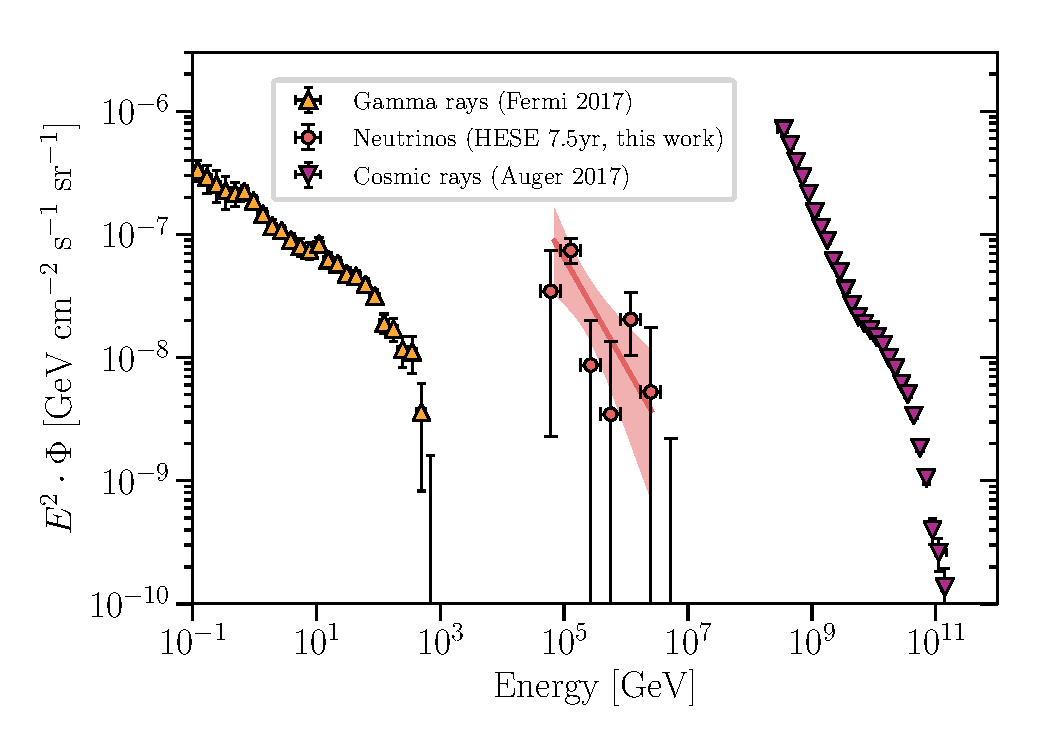
\includegraphics[width=\linewidth]{figures/hese_paper/astrophysical_overview}
	\internallinenumbers
	\caption{\textbf{\textit{High-energy fluxes of gamma rays, neutrinos, and cosmic rays.}}
		The segmented power-law neutrino flux, described in \refsec{sec:unfolding}, obtained in the analysis described in this paper is shown as red circles.
		The single power-law assumption, described in \refsec{sec:spl}, is shown as the light red region.
		The high-energy gamma-ray measurements by Fermi~\cite{Ackermann:2014usa} are shown in orange, while the very-high-energy cosmic-ray measurements by the Pierre Auger observatory~\cite{Fenu:2017hlc} are shown as purple data points.}\label{fig:all_cosmic}
\end{figure}